\documentclass{beamer}
\usepackage[english,francais]{babel}
\usepackage[T1]{fontenc}
\usepackage{lmodern}

%
% Choisir l'apparence de votre présentation.
%
% Pour plus de thèmes, de thèmes de couleur ou de thème de fontes, cf. :
% http://deic.uab.es/~iblanes/beamer_gallery/index_by_theme.html
%
\mode<presentation>
{
  \usetheme{Warsaw}       % ou essayer Darmstadt, Madrid, Dresden, ...
  \usecolortheme{default} % ou essayer albatross, beaver, crane, ...
  \usefonttheme{default}  % ou essayer serif, structurebold, ...
  \setbeamertemplate{navigation symbols}{}
  \setbeamertemplate{caption}[numbered]
} 

\title{Dédicace du cimetière de Gettysburg}
\author{Abraham Lincoln}
\institute{États-Unis d'Amérique}
\date{19 nov. 1863}

\begin{document}

\begin{frame}
  \titlepage
\end{frame}

\begin{frame}{Outline}
  \tableofcontents
\end{frame}

\section{Agenda}

\begin{frame}{Agenda}

\begin{itemize}
  \item Rencontré sur le champ de bataille (super)
  \item Part de terrain dédiée --- conforme !
  \item Travail non accompli (grands projets)
\end{itemize}

\end{frame}

\begin{frame}{Pas sur l'agenda !}

\begin{itemize}[<+->]
  \item Dédicace
  \item Consécration
  \item Creux (dans le sens étroit du mot)
  \item Addition ou rétractation
  \item Noter ou se souvenir de ce qui est dit
\end{itemize}

\end{frame}

\section{Critique}

\begin{frame}{Objectifs-clés \& facteurs de succès}

\begin{itemize}
\item Ce qui rend la nation unique :
  \begin{itemize}
  \item Conçue en liberté.
  \item Les hommes sont tous égaux.
  \end{itemize}
\end{itemize}

\begin{block}{Vision partagée}
\begin{itemize}
  \item Nouvelle naissance de la liberté.
  \item Gouvernement de/pour/par le peuple.
\end{itemize}
\end{block}

\end{frame}

\begin{frame}{Supervision organisationnelle}

\begin{figure}
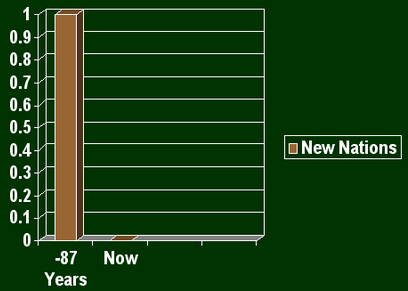
\includegraphics[width=0.5\textwidth]{gettysburg_graph}
\end{figure}

\begin{block}{Quatre fois vingt plus sept}
\begin{equation}
-(4 \times 20 + 7) = -87
\end{equation}
\end{block}

\end{frame}

\section{Résumé}

\begin{frame}{Résumé}

\begin{columns}
\begin{column}{0.4\textwidth}
\begin{itemize}
\item Nouvelle nation
\item Guerre civile
\item Terrain dédié
\end{itemize}
\end{column}
\begin{column}{0.6\textwidth}
\begin{itemize}
\item Dédicace au travail non accompli
\item Nouvelle naissance de la liberté
\item Gouvernement non périssable
\end{itemize}
\end{column}
\end{columns}

\end{frame}

\end{document}

